\section{Introduction} \label{section: intro and motiv}

\begin{wrapfigure}{r}{0.45\textwidth}
\vspace{-1.5cm}
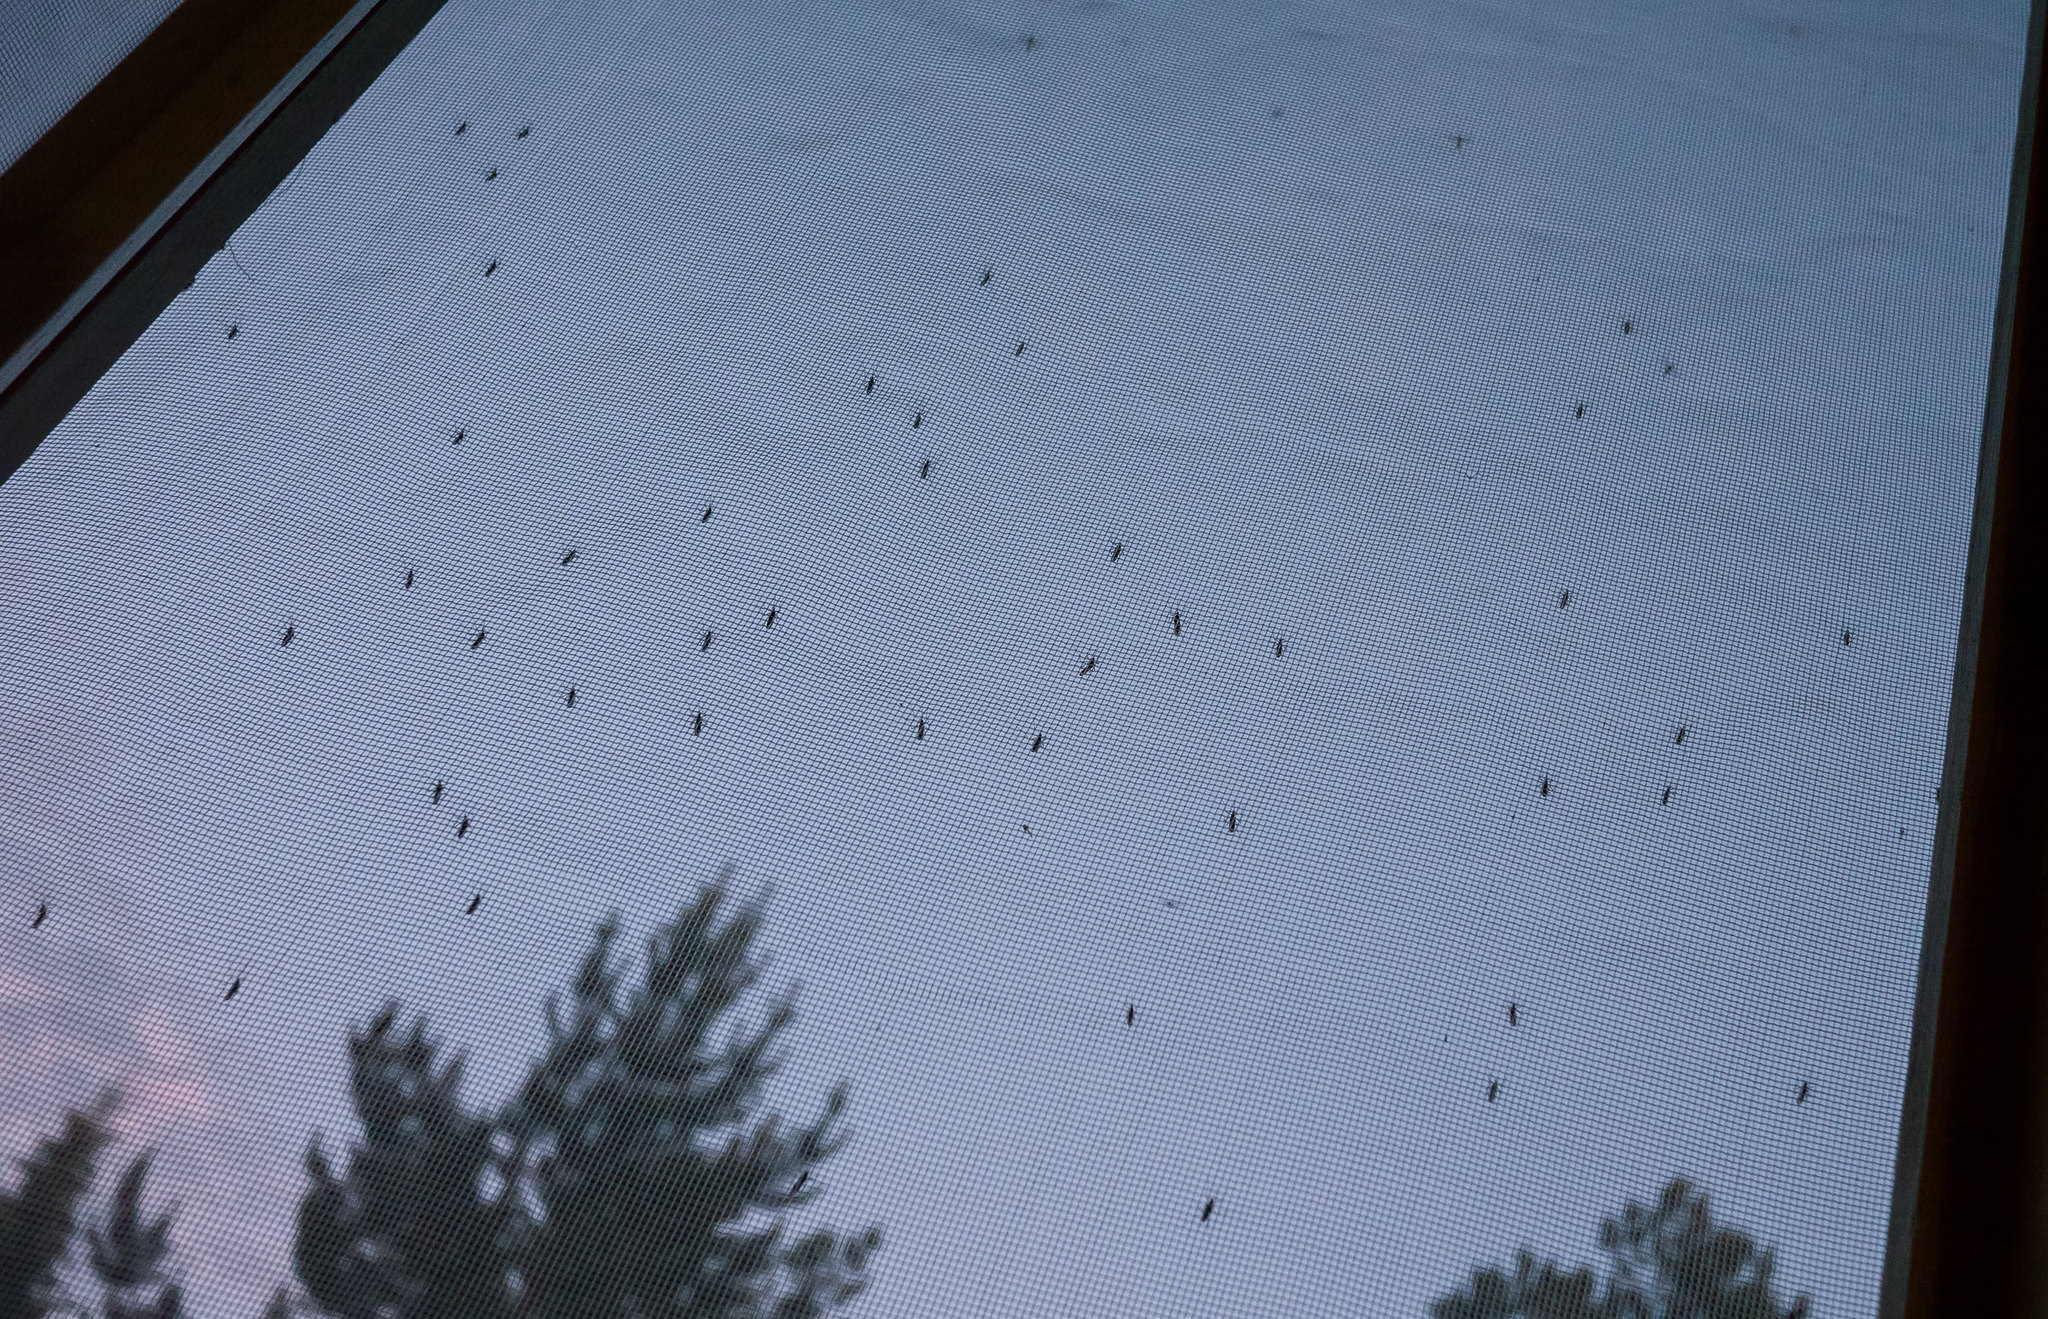
\includegraphics[width=0.9\linewidth]{figures/mosquitogrid.jpg}
\caption{Bug grid (\href{https://www.flickr.com/photos/neekohfi/7817306994/}{Flickr.com})}\
\end{wrapfigure}

Bug grids can be placed over open windows to allow air to flow through without letting bugs into someone's house. Presumably, when people open their windows, they want air to flow through their house. However, the installation of the grid decreases the functional cross-sectional area of the window, which might decrease the airflow. If the properties of the grid cause the flow to become turbulent, the reduction in airflow would be more drastic than due to the reduction in the cross-sectional area alone. Using a fluid simulation, this report aims to capture this phenomenon and investigate how the grid's thickness and density affect the airflow through a window. \\

To achieve this goal, a numerical simulation of airflow based on the Navier-Stokes equations was implemented in Python. The numerical simulation included discretising both space and time. The time discretisation was done using the Euler method, and the space discretisation was done using the finite difference method \cite{landau2015computational}. \\ 

In doing so, an investigation into the optimal parameters of the grid that maximise airflow while ``keeping the bugs out" was conducted. Additionally, the applicability and flexibility of fluid simulations in modelling real-world phenomena were demonstrated. Namely, the numerical stability and the computational efficiency of the simulation model were discussed. \\


\subsection{Research question}
% \textbf{Main:}
\begin{itemize}
    \item How much does the air flux through a window with a bug grid change with the grid's thickness and density?
\end{itemize}
% \textbf{Subquestions:}
% \begin{itemize}
%     \item What are the optimal parameters of the grid that maximise airflow while keeping the bugs out?
%     \item In which section of the window has the airflow decreased the most due to the presence of the bug grid?
% \end{itemize}

\subsection{Research goals}
\begin{itemize}
    \item Implement a numerical model for compressible fluid flow simulation.
    \item Investigate the effect of the bug grid's thickness (size of holes) and density (number of holes) on the airflow through a window.
    \item Determine if the bug grid introduces additional resistance to the flow of the fluid.
\end{itemize}